\documentclass[5p,authoryear]{elsarticle}
\makeatletter 
\def\ps@pprintTitle{%
 \let\@oddhead\@empty
 \let\@evenhead\@empty
 \let\@evenfoot\@oddfoot} % Supprimer le bas de page ELSEVIER
\makeatother
\usepackage[utf8]{inputenc} % En unicode
\usepackage[T1]{fontenc}
\usepackage[english]{babel}
\usepackage[babel=true]{csquotes} % permet de faire \enquote{a} (« a »)
\usepackage{amsmath} % pour certains signes mathématiques
\usepackage{amsthm} % Pour \begin{gather}
\usepackage{booktabs} % pour \toprule (un style de tableau)
\usepackage{multirow} % Pour colonnes multiples des tableaux
\usepackage{amssymb} % Pour \leqslant (<=, >=)
\usepackage{float}
\usepackage{hyperref} % 
\usepackage[english]{cleveref} 

% adding Code Blocking
\usepackage{listings}
\usepackage{color}

\definecolor{dkgreen}{rgb}{0,0.6,0}
\definecolor{gray}{rgb}{0.5,0.5,0.5}
\definecolor{mauve}{rgb}{0.58,0,0.82}

\lstset{frame=tb,
  language=Java,
  aboveskip=3mm,
  belowskip=3mm,
  showstringspaces=false,
  columns=flexible,
  basicstyle={\small\ttfamily},
  numbers=none,
  numberstyle=\tiny\color{gray},
  keywordstyle=\color{blue},
  commentstyle=\color{dkgreen},
  stringstyle=\color{mauve},
  breaklines=true,
  breakatwhitespace=true,
  tabsize=3
}




%\bibliographystyle{elsarticle-num}
\bibliographystyle{elsarticle-harv}

\usepackage{fancyhdr}
\pagestyle{fancy}
\lhead{MSDS 458 - SEC 56}
\rhead{Lee, J.}

\begin{document}

\begin{frontmatter}

\title{Computer Vision: \\Single Hidden Layer Neural Network Analysis}
\author{Jason Lee}
\address{Northwestern University, SPS \\Artificial Intelligence and Deep Learning \\2019FA MSDS 458-56}


\begin{abstract}
Artificial neural networks are commonly known as “black-box” algorithms. 
This paper takes a look inside the black box to understand how a neural network actually learns from the input data. 
To do this, a very simple classification problem will be used. 
The focus of the analysis will be on the subtle differences found within the node weights that occur by changing the number of nodes in a single hidden layer neural network. 
The goal is to determine what these hidden nodes are responding to in the training data to reach the final prediction.
\end{abstract}


\begin{keyword}
Neural Networks \sep Computer Vision \sep Deep Learning \sep Letter Recognition 
\end{keyword}

\end{frontmatter}


\section{Introduction}\label{introduction}


There is growing popularity surrounding the topics of deep learning, computer vision, and neural networks over the last several years. As data scientists, it is our responsibility to understand exactly how the different algorithms we use each day actually work, including the “black-box” algorithms like neural networks. 
There may be a situation when a data scientist is asked to develop a neural network prediction model for letter classification. 
Knowing how to go about training such a model and evaluating its effectiveness is crucial if the model is expected to be deployed with confidence in the real world. 

Contrary to popular belief, an artificial neural network does not work the exact same way as the human brain \citep{chollet}, but these algorithms were inspired by how the brain learns \citep{goodfellow}. 
A neural network is a mathematically dependent model that receives input data and produces an output based on strict mathematical rules. 
These models are able to improve, or learn, over the course of their training time as internal weights are updated in a feedback loop.

Deep neural networks (DNNs) are extremely powerful and incredibly intricate. 
They have proven to be effective solving previously unsolvable, complex problems, such as speech recognition, natural language processing, and image recognition. 
Undoubtedly, these models still follow the same strict mathematical rules as simpler neural networks. 
In order to understand how deep neural networks work, it is recommended to start exploring shallow neural networks with only a single hidden layer.

The purpose of this analysis is three-fold:
\begin{enumerate}
 \item Exploring neural networks with a simple dataset to investigate how they learn from the input data.
 \item Examine what happens when adjusting the number of nodes in a single hidden layer structured neural network.
 \item Creating a reproducible Python prediction model to easily share with colleagues. 
\end{enumerate} 


\subsection{Letter Recognition}

To accomplish the goals of this analysis, the English language alphabet will be used as the training dataset for the computer vision model. 
This dataset has only 26 rows, a single observation for each letter in the alphabet. 
The letters are arranged as 9x9 pixel images consisting of binary values signifying whether or not the individual pixel is activated. 
There are 26 classes, one for each letter, that the neural network will need to differentiate between when reaching its final prediction. 
This use case will be relatively simple in order to explore the changes in the weights when adjusting the number of nodes in the models.


\section{Literature Review}\label{lit_rev}

There has been substantial research completed around neural networks. 
It is important to understand how a very simple artificial neural network is trained. 
There are obviously inputs at the start of the model and an output at the end. 
There are a few other key aspects of a neural network. 
Inside the network there are hidden layers, in each hidden layer there are nodes, each node has weights augmenting the data that it receives. 
The diagram in Figure \ref{basic} below helps visualize the network structure \citep{Python}.\\

\begin{figure}[!htb] \centering
	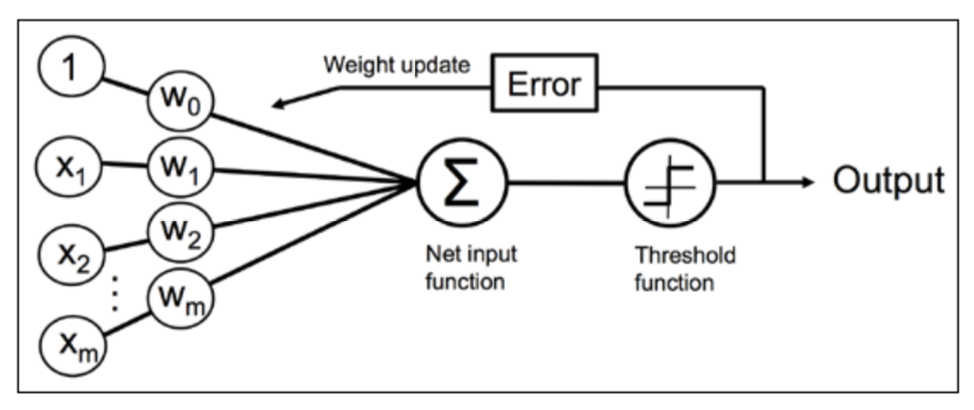
\includegraphics[width=3.4in]{figures/Figure nn.png}
	\caption[]{Basic Neural Network Diagram} 
	\label{basic} 
\end{figure}

The input data of the model are run through each layer and node to produce an output, or prediction. The neural network’s predictions are then compared to their true label. The error metric, or objective function that is being optimized in the model, is calculated (2017). The model may start with a very inaccurate prediction with a large error metric; however, the training process is not complete.

The neural network learning process utilizes a forward-feed through the layers and then a backpropagation process through each of the layers in reverse. When the error metric is calculated, the network works backwards taking partial derivatives of the loss function updating the internal weights of each node utilizing the chain rule \citep{brownlee}. A full loop, forward pass and backward pass, through the neural network is known as an epoch. After each epoch, the error metric should decrease as the accuracy of the model improves. 

Neural networks can fall into a trap where they actually memorize the training dataset. This is common when there are more weights than training samples. This will make the prediction model ineffective when trying to predict on a new dataset [6]. To mitigate this issue, bias and nonlinear activation functions are used making the model able to generalize and adapt to new observations (Brownlee, 2019).



\section{Methodology}\label{meth}

The methodology utilized in this analysis followed a relatively simple approach similar to Gorman and Sejnowski \citep{gorman}. 
There will be five distinct neural networks trained. 
The key difference between the models will be the number of nodes contained within the single hidden layer. 
By increasing the number of nodes, a comparison can be made showing how each model extracts important aspects of the input images to differentiate between the letters. 

The Keras package in Python, which is built on TensorFlow, will be used to develop each of the five neural networks. 
The training process for each neural network will run for a total duration of 2,500 epochs. 
The hidden layer will use a rectified linear unit (ReLU) activation function and the output layer will use the softmax activation function.


\subsection{Neural Network Architecture}\label{arch}

There will be only one fully connected, or dense, hidden layer for all of the neural network’s topology. 

\subsubsection{Nodes}\label{corpus}


There are five different node variations: 

\begin{enumerate}
 \item 2 Nodes – This model will have 242 trainable parameters, 164 in the hidden layer and 78 in the output layer.
 \item 3 Nodes – This model will have 350 trainable parameters, 246 in the hidden layer and 104 in the output layer. 
 \item 4 Nodes – This model will have 458 trainable parameters, 328 in the hidden layer and 130 in the output layer.
 \item 13 Nodes – This model will have 1,430 trainable parameters, 1,066 in the hidden layer and 364 in the output layer.
 \item 26 Nodes – This model will have 2,834 trainable parameters, 2,132 in the hidden layer and 702 in the output layer.
\end{enumerate} \\


\subsubsection{Optimization Function}\label{opt}

The optimization function for the neural networks will be the RMSProp in the Keras’ package. The RMSProp optimization method adjusts the learning rate during the training process by dividing the gradient by the running average of its recent magnitudes. This will help speed up the training process utilizing momentum (2018). 


\subsubsection{Loss Function}\label{loss}

The loss function employed in each neural network for this analysis was the categorical cross-entropy function because there are 26 categorical outcomes in the model. The categorical cross-entropy method follows the form \citep{mool}:
\begin{equation}
    Loss = -\sum_i^n{y_i\log_2 y_i}
\end{equation}


\subsection{Dataset}\label{data}

The dataset used in this analysis was provided by Dr. Miller in the course assignment starter code \citep{sample-code}. 
The dataset consists of 26 alphabetic characters in small 9x9 image grids. 
This small and simple dataset has been selected purposefully to accomplish the key goals of this analysis. 
Figure \ref{abc} below shows examples of how the computer visualizes the first three and last three letters in the dataset. 

\begin{figure}[!htb] \centering
	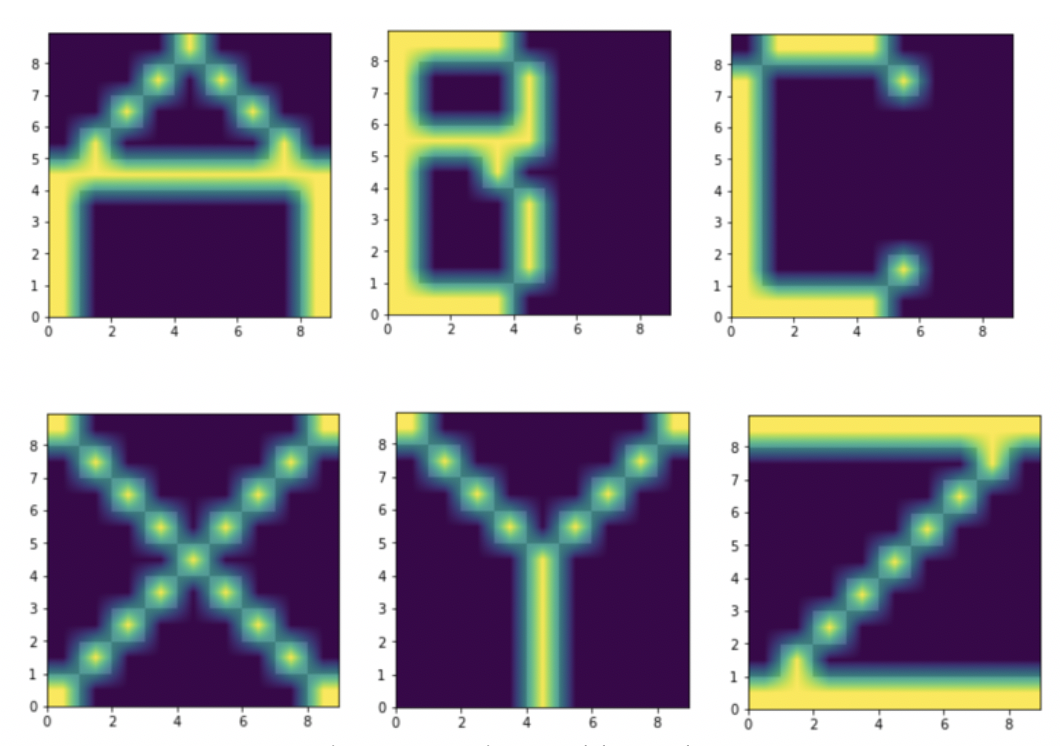
\includegraphics[width=3.4in]{figures/abc_xyz.png}
	\caption[]{First 3 and last 3 letters in the dataset visualized how the algorithm "sees" them.} 
	\label{abc} 
\end{figure}

The dataset has been transformed and split into input variables and a target variable to feed into the neural networks. 


\subsubsection{Input Data}\label{input}

The input data of 26 9x9 image grids for the neural networks have each been flattened into single row observations with 81 features, one for each pixel in the image. 
Each of the 81 features is a binary variable, one for an activated pixel and zero for dormant pixel. 

The composite image grid of our training dataset looks like this:

\begin{figure}[!htb] \centering
	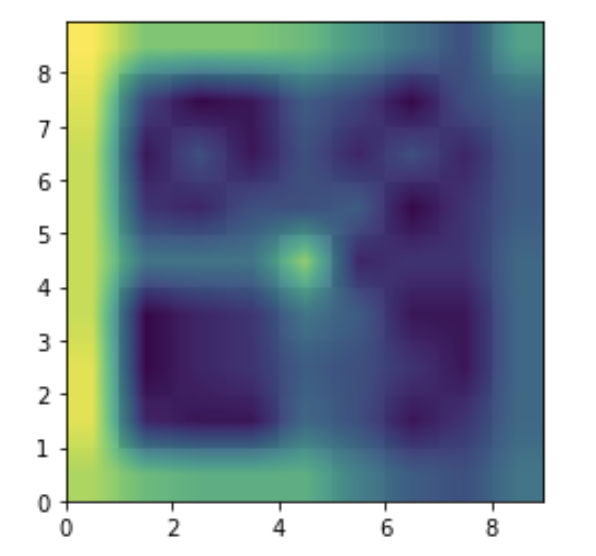
\includegraphics[width=3in]{figures/All Letters.png}
	\caption[]{All letters activated} 
	\label{abc} 
\end{figure}


As can be seen from the image, there are certain areas that are highly populated, particularly the first column along the left-hand side of the image. 
There are also several letters that show positive signals in the first and last rows up until about the fifth or sixth column. 
The center of the image also appears heavily populated. 

The models will be able to learn how to differentiate between the various letters by extracting unique combinations of these features in each node. 
A node in the model may pick up signal areas that are less populated, or more unique for that particular letter. 
For example, the letter “Z” is the only letter that has the entire first and last column completely populated. 
Exploring the weights of a trained model will help one see which areas are more important for each node. 


\subsubsection{Target Data}\label{input}

This particular modeling goal is a classification problem. 
The target variable is a categorical variable with 26 different classes, one for each letter in the alphabet. 
Neural networks need to have numeric inputs and outputs for them to work. 
Data manipulation and transformations are needed for the model to solve this problem.

A Keras’ function called “LabelEncoder” was utilized to transform the letters into a numeric array ranging from 0 to 25 assigning a number to each individual letter. 

There was one final preparatory step needed to transform the target data for modeling. 
Another Keras’ function “to\_categorical” was used to create a binary matrix. 
This matrix has a shape of 26x26 where each row is populated with 25 zeros and a single one value corresponding to the class it represents. 
Now the target data is ready for use in the various models.




\section{Computational Experiment}

The Python code for the analysis performed here can be reproduced using \href{https://colab.research.google.com/drive/18ETB63048EzJToFIklG0F_-shNV5fHF7}{Google Collaboratory Notebook} at this url:

\begin{displayquote}
\centering
\href{https://colab.research.google.com/drive/18ETB63048EzJToFIklG0F_-shNV5fHF7}{Notebook LINK}
\end{displayquote}

The Python Notebook walks through each step and each model.  


\section{Results}

\subsection{Neural Network 1: 2 Hidden Nodes}\label{one}

The first neural network trained only has 2 nodes in the hidden layer. 
Figure \ref{test1a} visualizes the model with the input features in green, hidden layer’s nodes in blue, and the output classes in red. 
Figure \ref{test1b} gives a summary of the model and the total number of parameters that have been adjusted during the training process.

\begin{figure}[!htb] \centering
	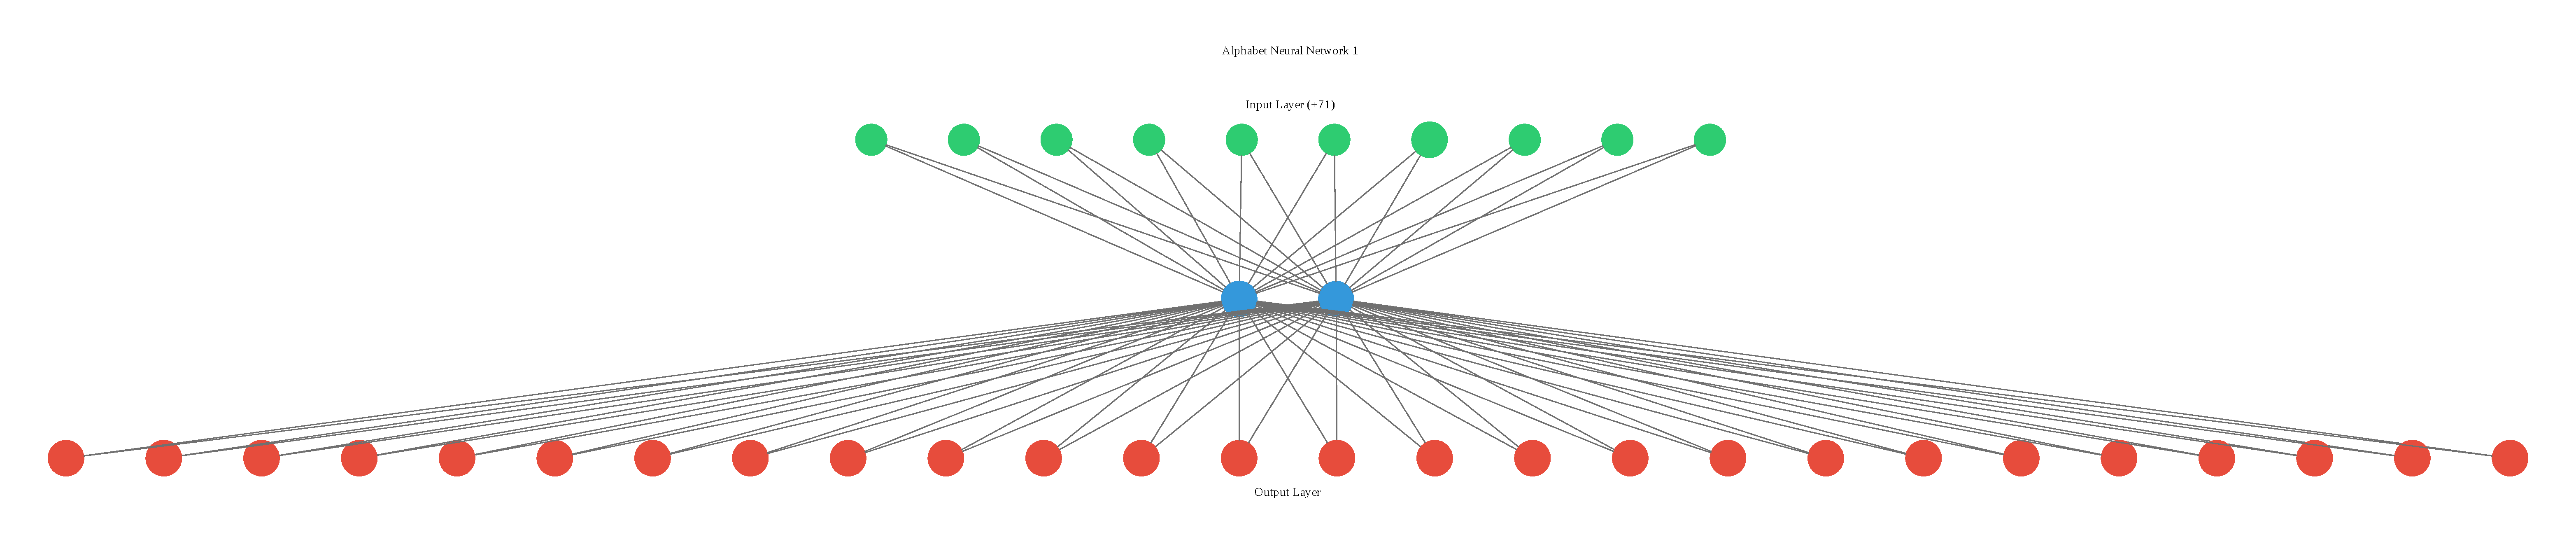
\includegraphics[width=3.4in]{figures/nn1.pdf}
	\caption[]{Neural Network 1 Architecture} 
	\label{test1a} 
\end{figure}


\begin{figure}[!htb] \centering
	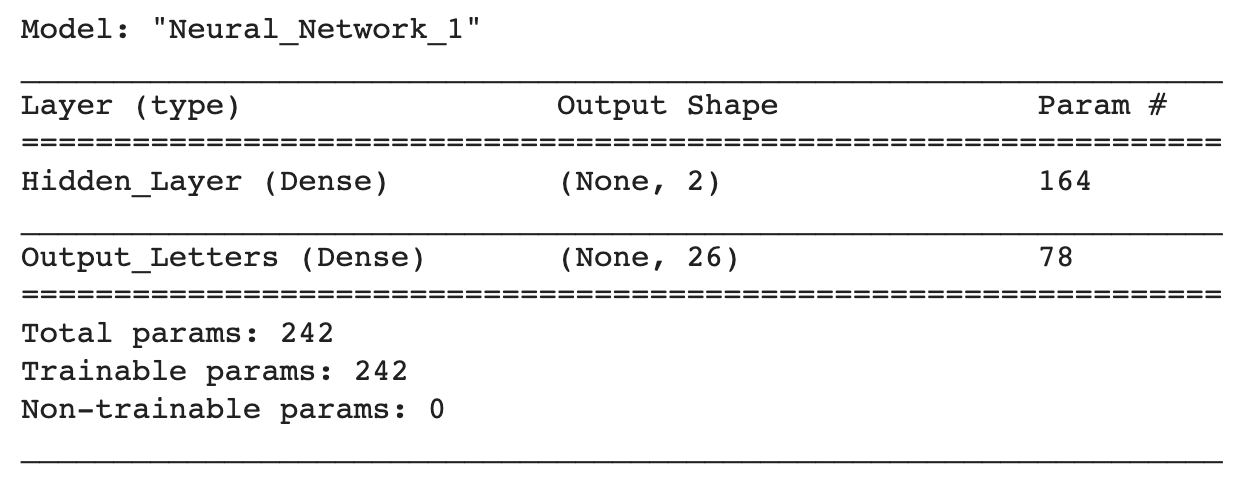
\includegraphics[width=3.4in]{figures/nn1 sum.png}
	\caption[]{Neural Network 1 Model Summary} 
	\label{test1b} 
\end{figure}

\begin{figure}[!htb] \centering
	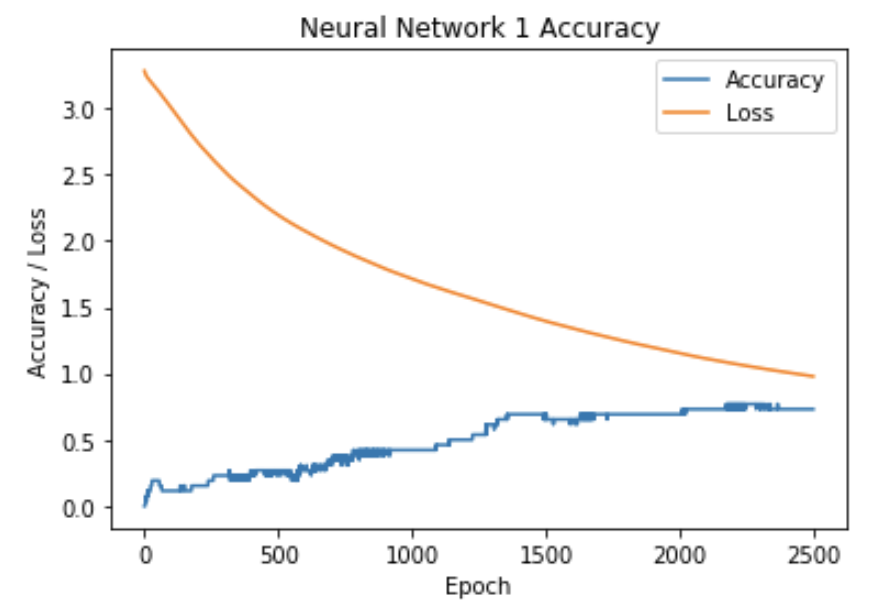
\includegraphics[width=3.4in]{figures/nn1 plot.png}
	\caption[]{Neural Network 1 Training Results} 
	\label{test1c}
\end{figure}

As one can see in Figure \ref{test1c}, this model reached a maximum accuracy of 73.08\% over the course of 2,500 epochs in a training time of 12.66 seconds. 
Because there are 26 different classes the model is trying to predict, it is more difficult for it to achieve a high predictive accuracy quickly with only 2 nodes. 
The directionality of the slope of both the loss and accuracy curves suggest that given a longer training time this model could reach better results. 

\begin{figure}[!htb] \centering
	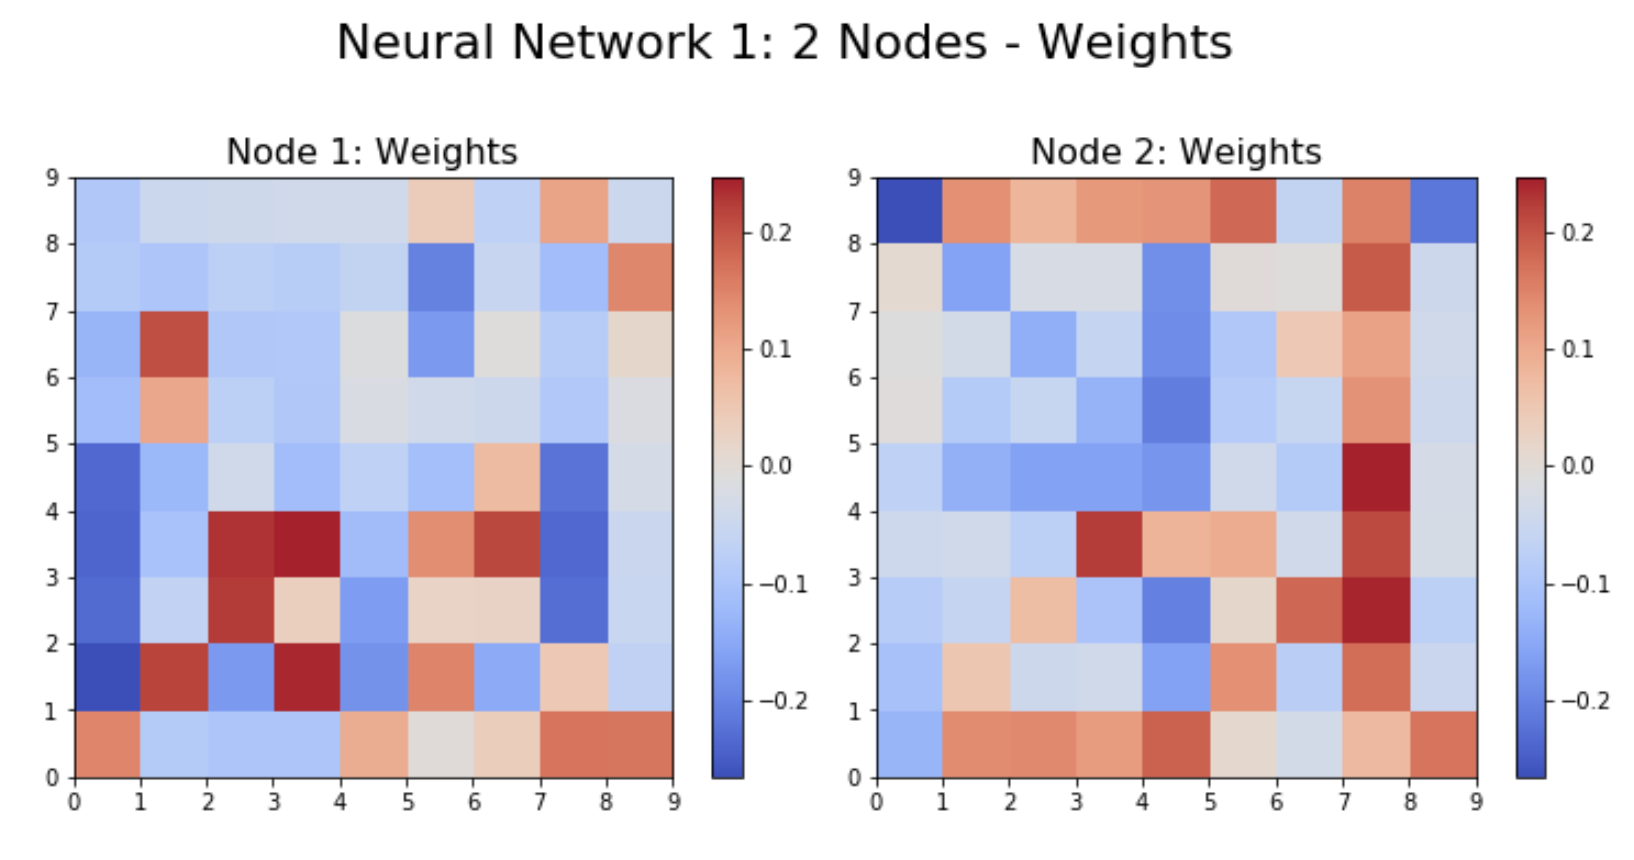
\includegraphics[width=3.4in]{figures/nn1_weights.png}
	\caption[]{Neural Network 1 Node Weights} 
	\label{test1d}
\end{figure}

This model’s weights are featured in Figure \ref{test1d}. 
This plot shows where the node has positive (red) and negative (blue) values for each input variable. 
It appears that Node 1 has less activations in the top half compared to the bottom half. 
The bottom left diagonal [(1,1), (2,2), (3,3), (4,4)] all have very positive weights. 
There are strong negative weights in the bottom half of the 1st column. 

Node 2 has strong positive activations across the entire 8th column and more neutral values on the left-hand side. 
When comparing Node 1 and Node 2, there are very few areas that have overlapping weights. 


\subsection{Neural Network 2: 3 Hidden Nodes}\label{two}

The number of nodes in the hidden layer has been increased from 2 to 3 for this neural network. 
Figure \ref{test2a} shows a very similar structure as the first with the only difference being one addition blue node in the hidden layer. 
The increase of one node increased the total number of trainable parameters by 45\%.

\begin{figure}[!htb] \centering
	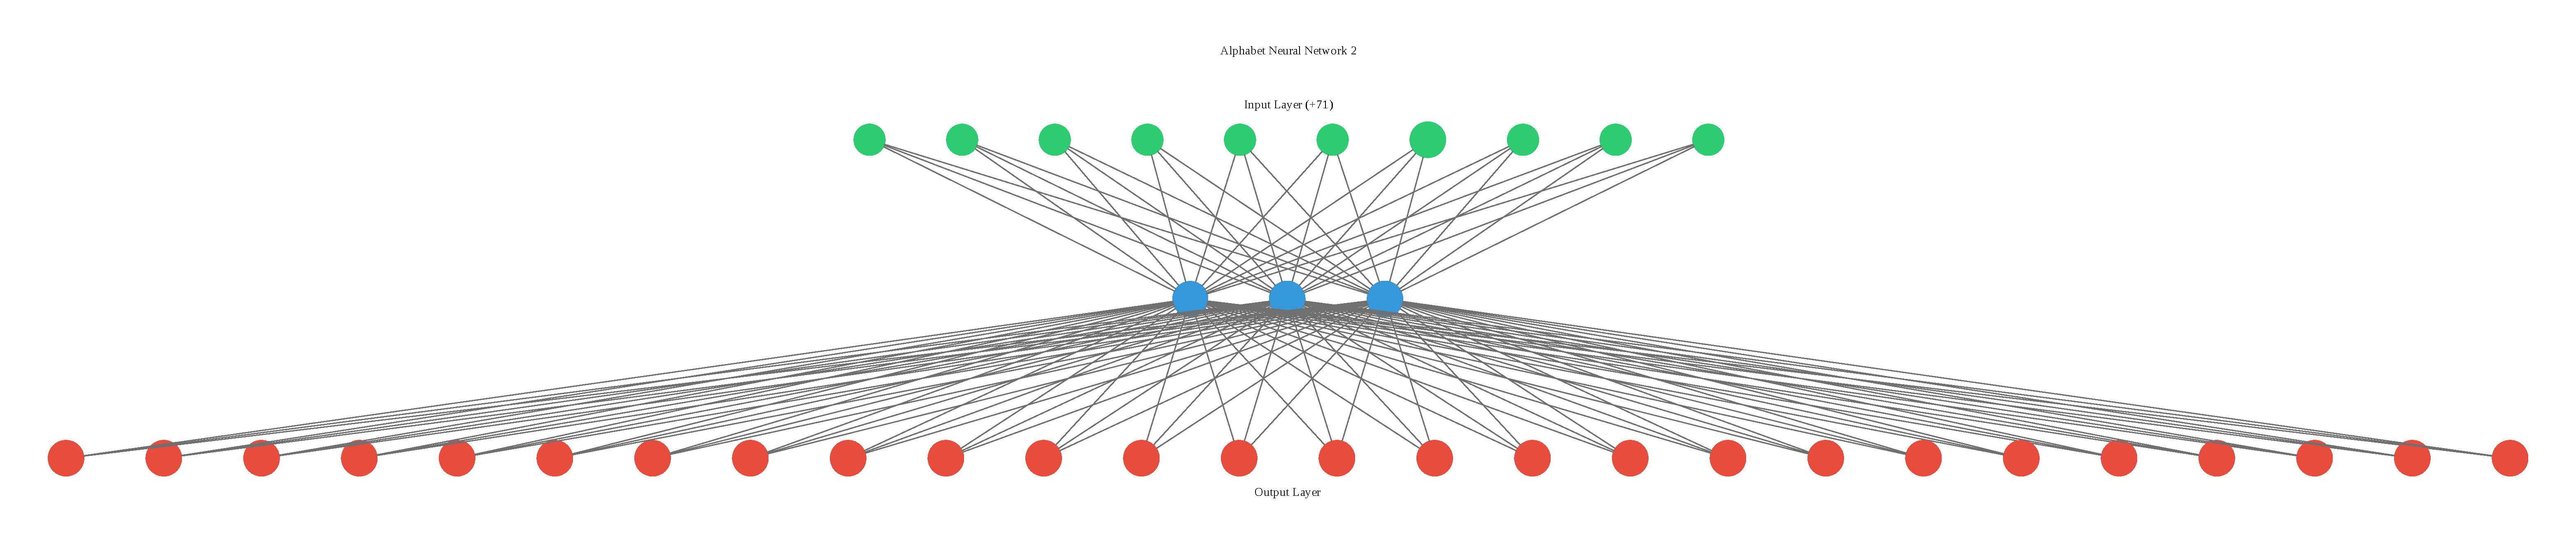
\includegraphics[width=3.4in]{figures/nn2.pdf}
	\caption[]{Neural Network 2 Architecture} 
	\label{test2a} 
\end{figure}


\begin{figure}[!htb] \centering
	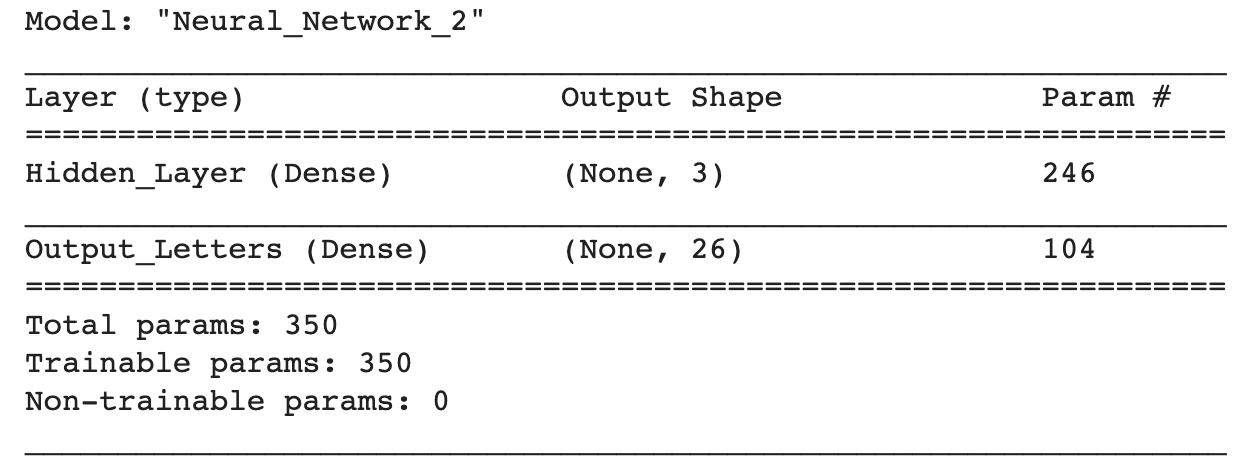
\includegraphics[width=3.4in]{figures/nn2 sum.png}
	\caption[]{Neural Network 2 Model Summary} 
	\label{test2b} 
\end{figure}

\begin{figure}[!htb] \centering
	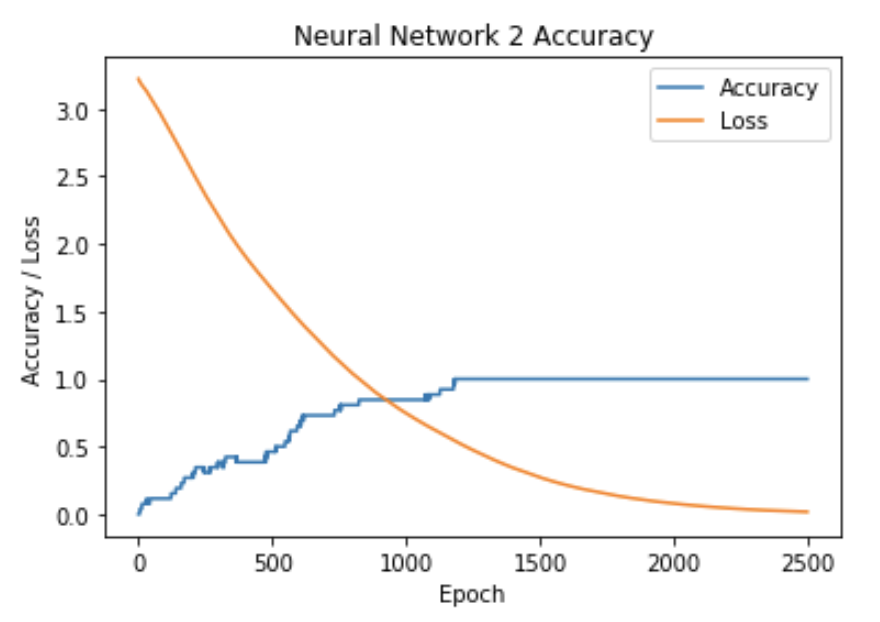
\includegraphics[width=3.4in]{figures/nn2 plot.png}
	\caption[]{Neural Network 2 Training Results} 
	\label{test2c}
\end{figure}

This model achieved 100\% accuracy before the 2,500 epochs of training. 
It only took 1,182 epochs to achieve perfection. 
The total training time was 10.33 seconds for this model.

\begin{figure}[!htb] \centering
	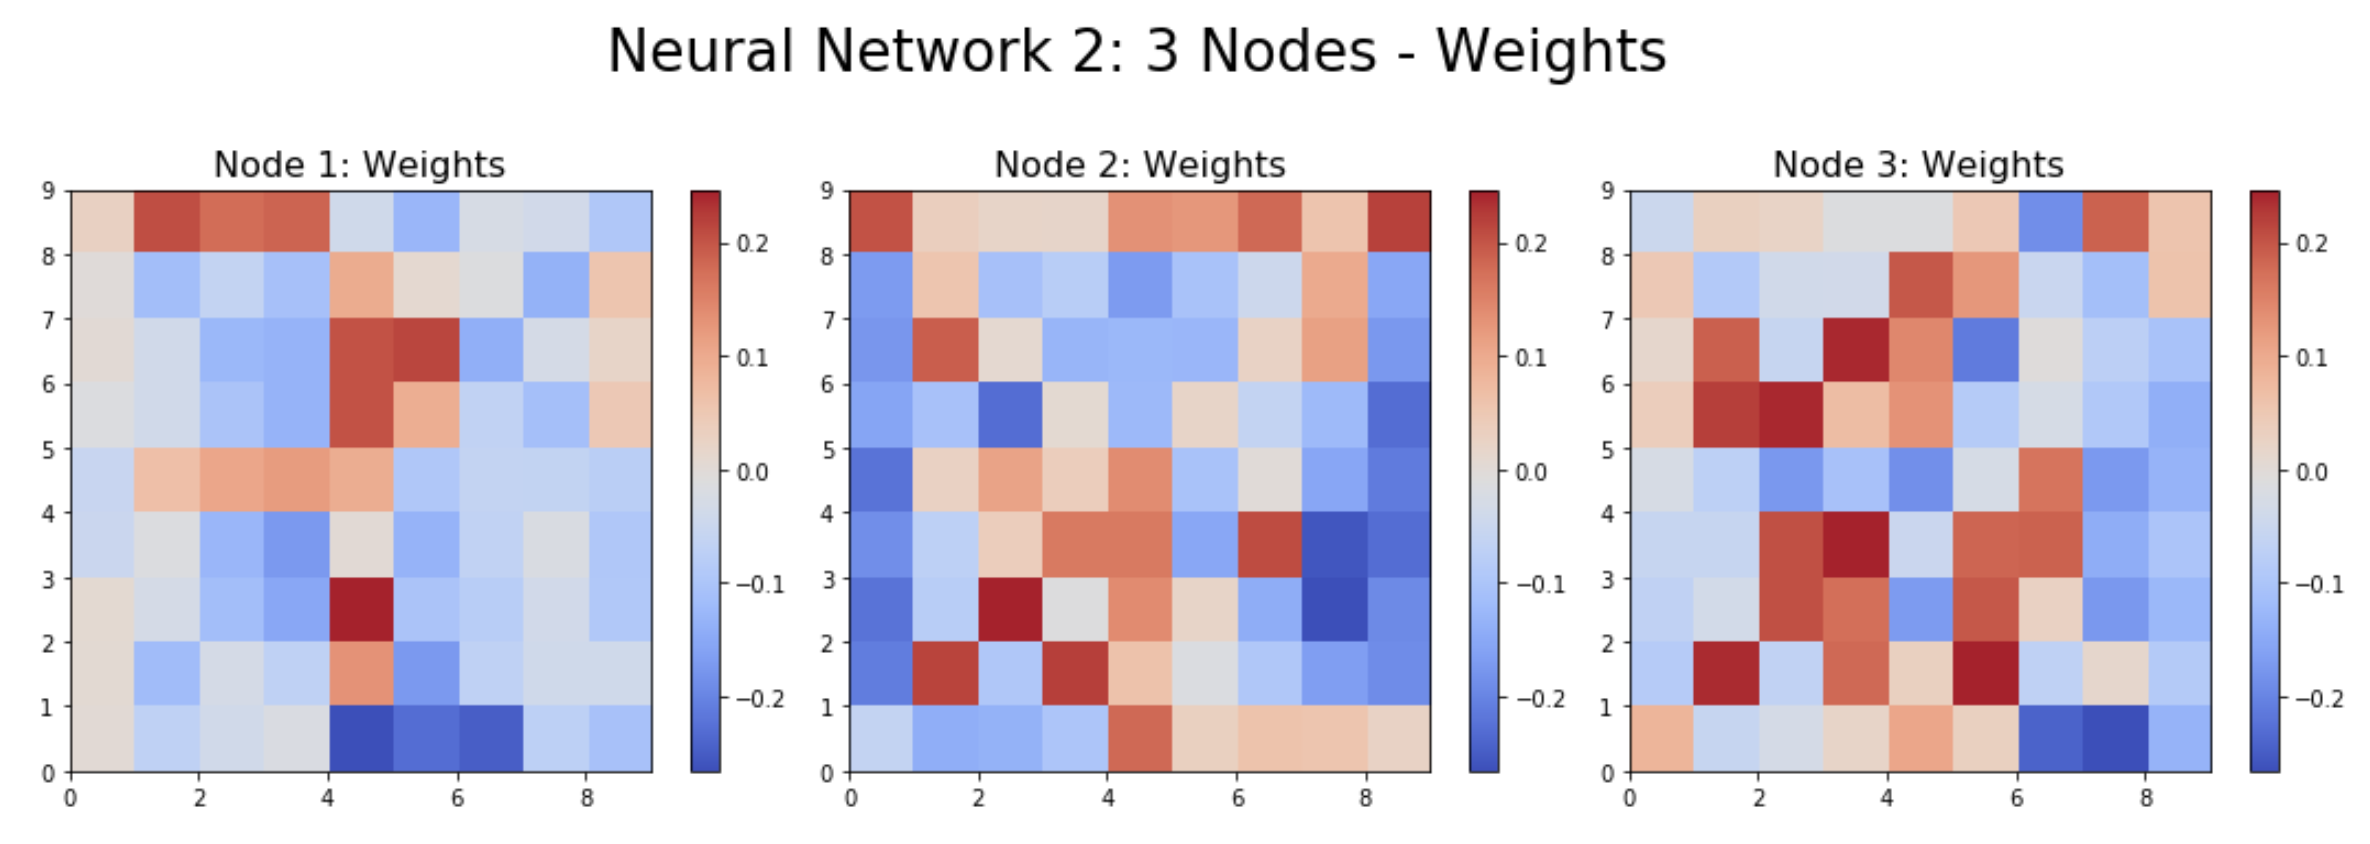
\includegraphics[width=3.4in]{figures/nn2_weights.png}
	\caption[]{Neural Network 2 Node Weights} 
	\label{test2d}
\end{figure}

This model’s weights for the three nodes are visually presented in Figure \ref{test2d}. 
Node 3’s bottom half weights look very similar to node 1 in our first model. 
That same diagonal pattern in the bottom left is weighted heavily here too. 

Node 1 appears to be relatively neutral in most of the input areas. 
The main activations are directly down the center of the plot. 
There is also a pocket of strong negative weight in [(1,5), (1,6), (1,7)] and strong positive weights at the top [(9,2), (9,3), (9,4)].
The top two corners in node 2 are important positive weights. There is also some overlap between node 2 and 3 in several areas.

The third node in this model appears to have the largest magnitude summed across the entire input space, both positive and negative. 
There are many areas of negative and strong positives. 



\subsection{Neural Network 3: 4 Hidden Nodes}\label{one}

Taking the next step in this analysis by increasing the number of nodes in the hidden layer from 3 to 4, Figure \ref{test3a} and Figure \ref{test3b} show the new model structure and model summary. 
This node increase upped the total number of trainable parameters by 31\%. 
The model now has 458 parameters that will be tweaked during the training process to reach the final prediction. 

\begin{figure}[!htb] \centering
	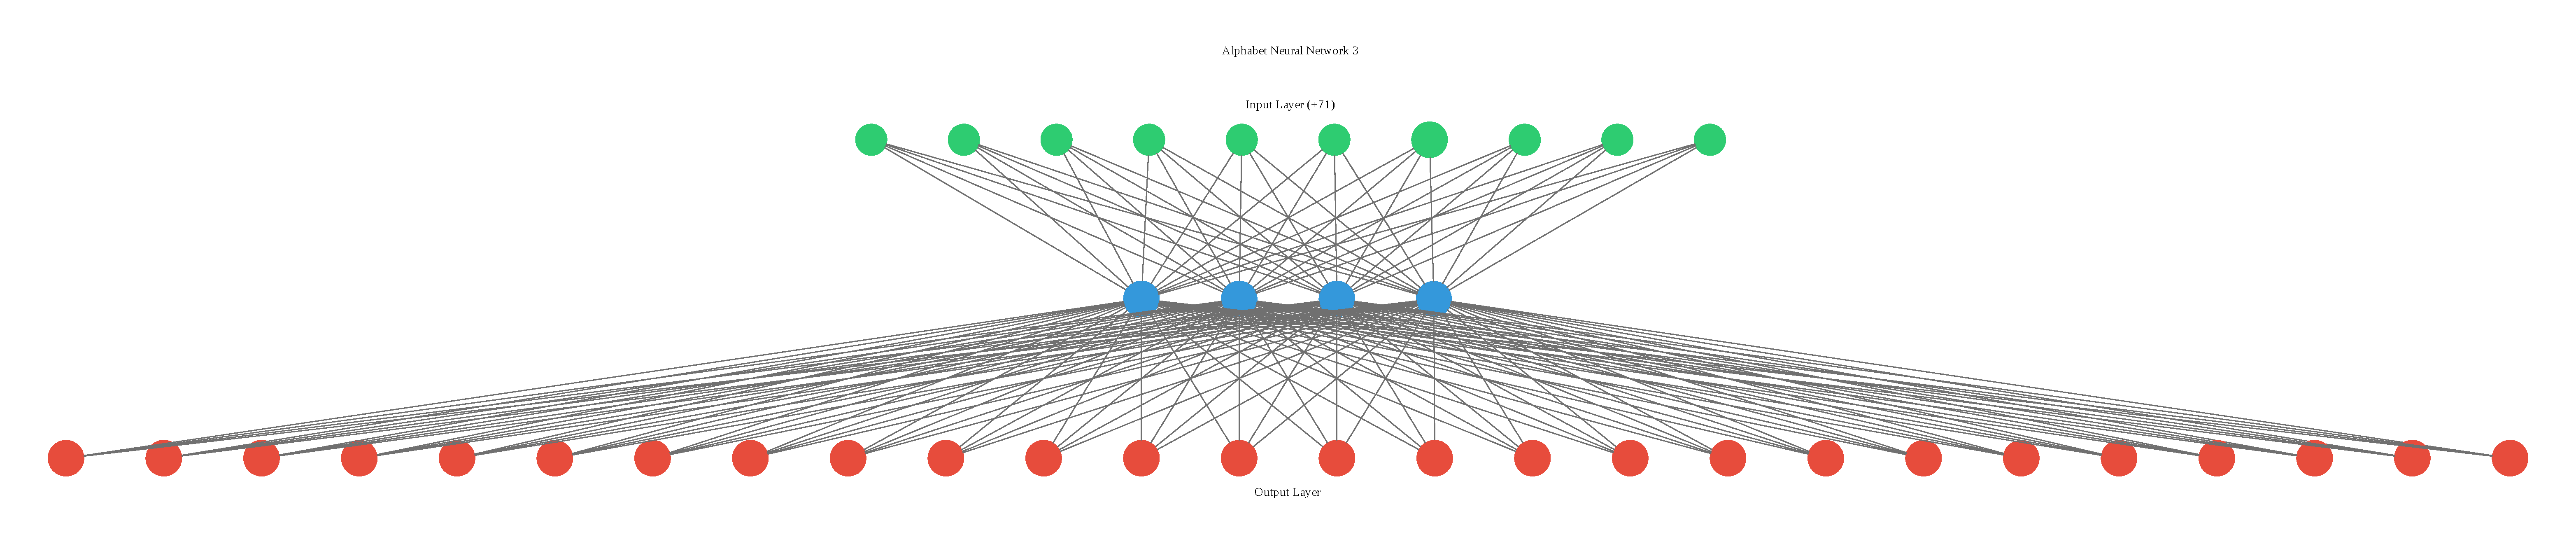
\includegraphics[width=3.4in]{figures/nn3.pdf}
	\caption[]{Neural Network 3 Architecture} 
	\label{test3a} 
\end{figure}


\begin{figure}[!htb] \centering
	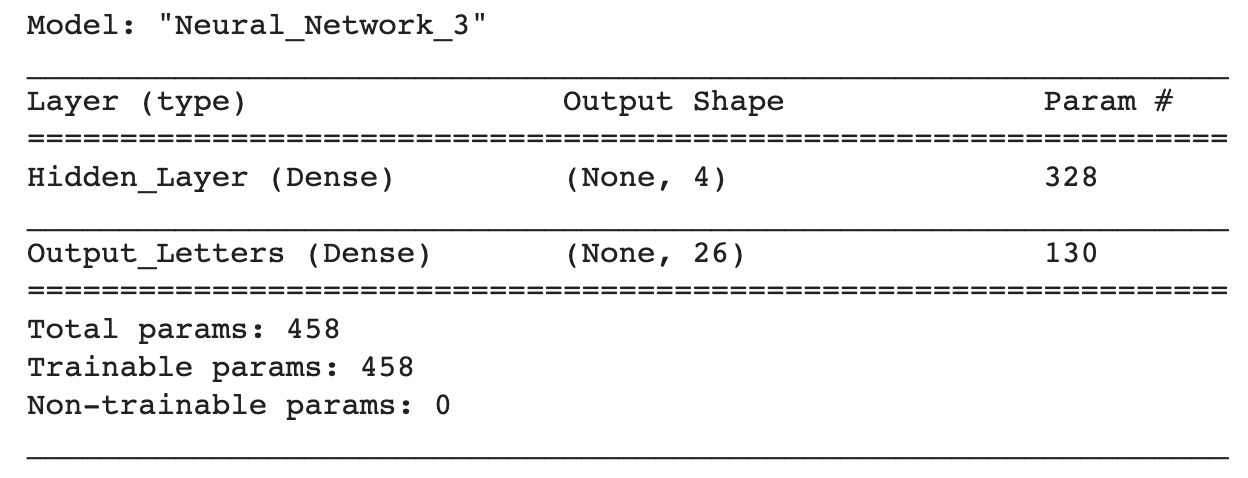
\includegraphics[width=3.4in]{figures/nn3 sum.png}
	\caption[]{Neural Network 3 Model Summary} 
	\label{test3b} 
\end{figure}

\begin{figure}[!htb] \centering
	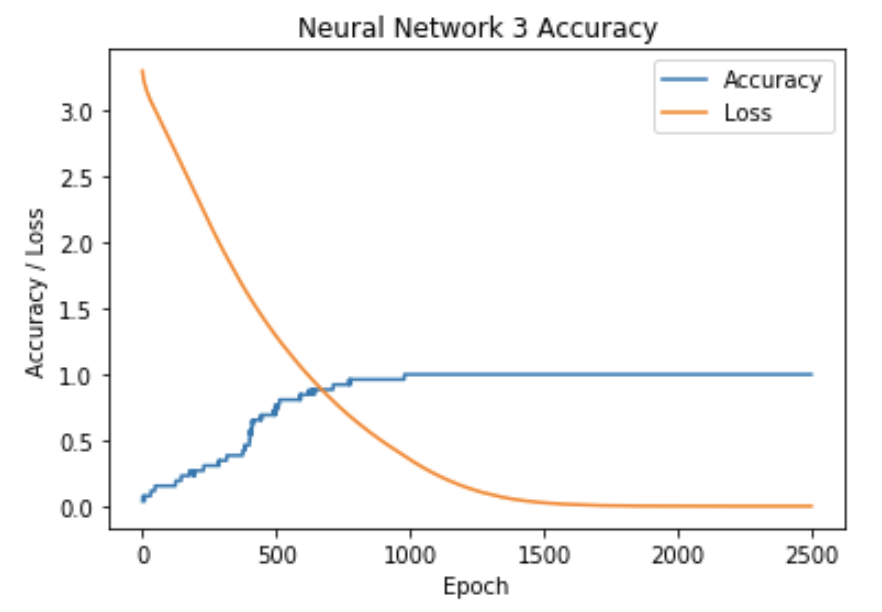
\includegraphics[width=3.4in]{figures/nn3 plot.png}
	\caption[]{Neural Network 3 Training Results} 
	\label{test3c}
\end{figure}

This model reached 100\% accuracy in 980 epochs, a 17\% decrease from our last model. 
The total training time clocked in at 12.38 seconds through the 2,500 epochs.

\begin{figure}[!htb] \centering
	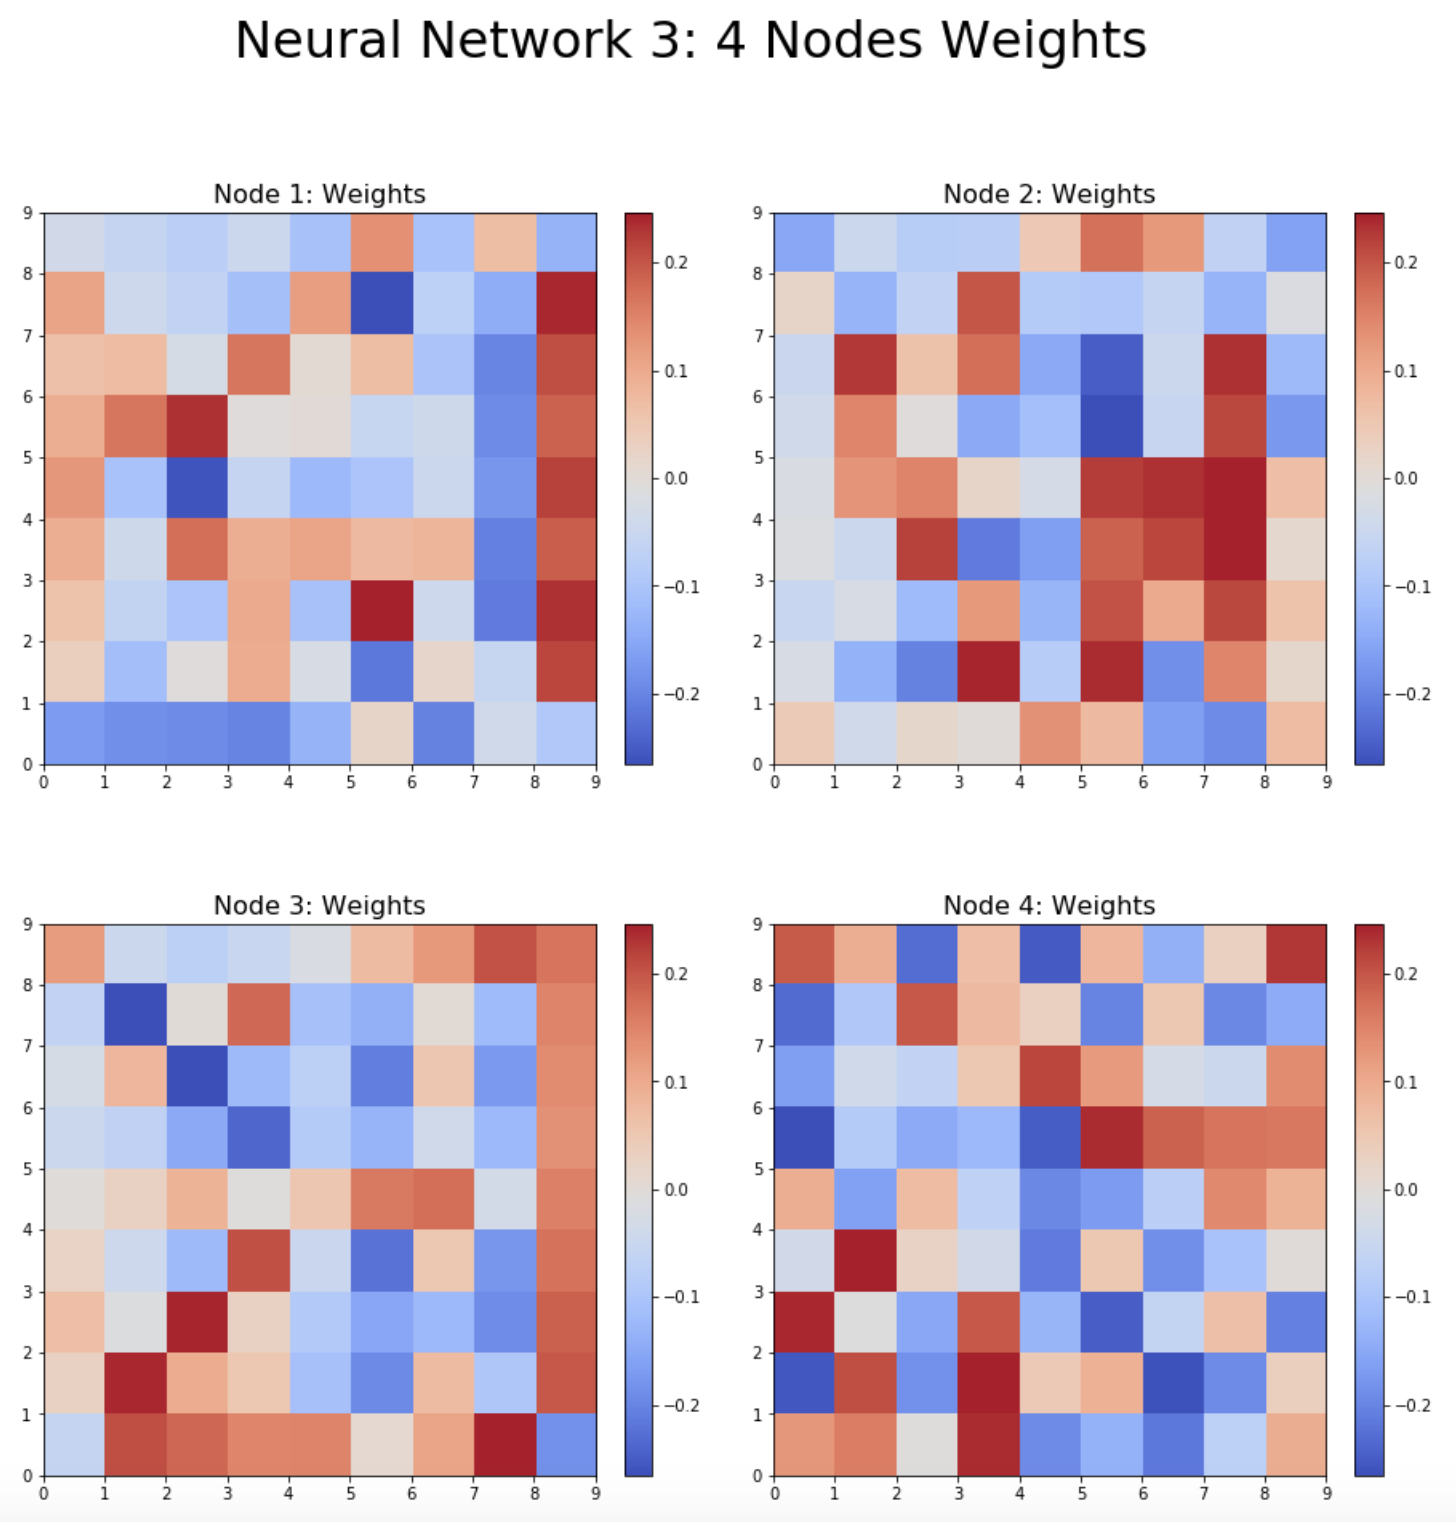
\includegraphics[width=3.4in]{figures/nn3_weights.png}
	\caption[]{Neural Network 3 Node Weights} 
	\label{test3d}
\end{figure}

The weights for each of the nodes in this model in Figure \ref{test3d} appear to be more dispersed across the 81 inputs. 
Each node has their most heavily weighted areas in different locations with very few overlaps. 
Node 1 covers the last column, while node 2 has heavy positive weights in the second to last column. 
Node 3 captures the importance of the bottom left diagonal that we have consistently seen in previous models. 


\subsection{Neural Network 4: 13 Hidden Nodes}\label{one}

After increasing the models by a single node each time, there is a need to explore how the weights reacted when there were half as many nodes as output classes. 
This neural network has 13 nodes in the hidden layer. 
The number or trainable parameters in this model is now 1,430. 
This should allow the neural network more flexibility in feature extraction than the other models.

\begin{figure}[!htb] \centering
	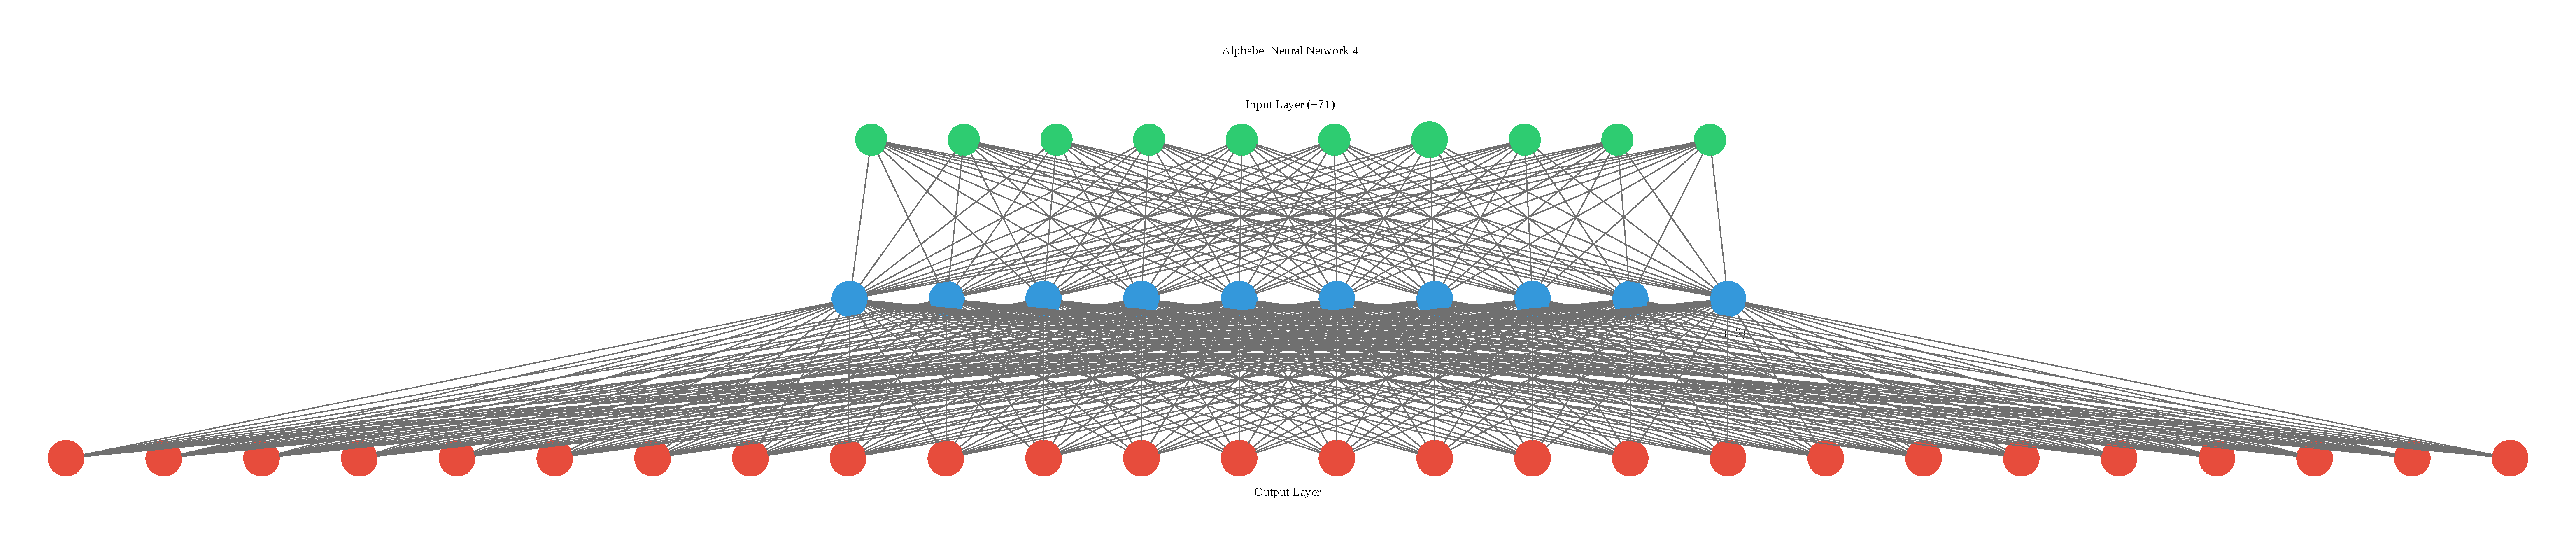
\includegraphics[width=3.4in]{figures/nn4.pdf}
	\caption[]{Neural Network 4 Architecture} 
	\label{test4a} 
\end{figure}


\begin{figure}[!htb] \centering
	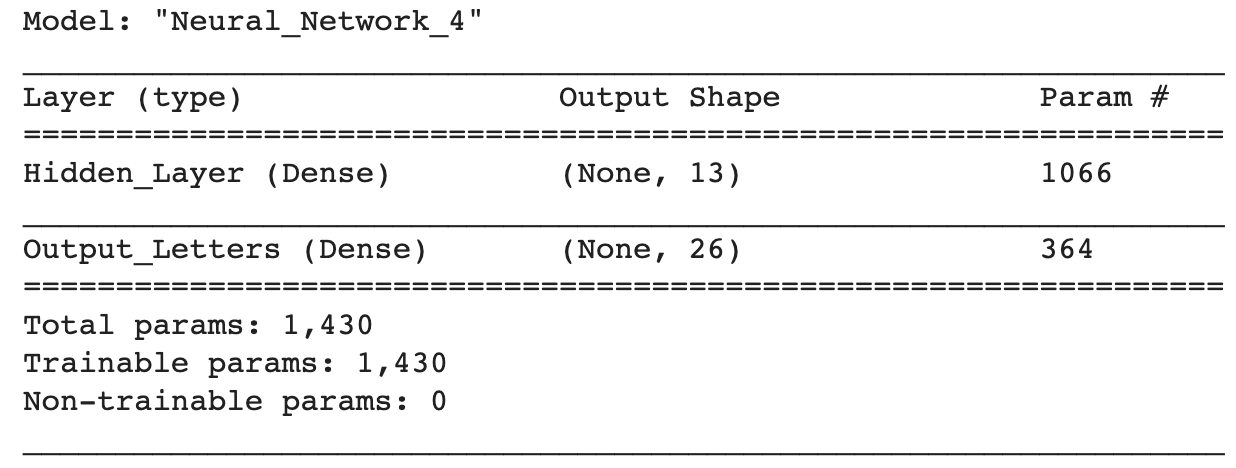
\includegraphics[width=3.4in]{figures/nn4 sum.png}
	\caption[]{Neural Network 4 Model Summary} 
	\label{test4b} 
\end{figure}

\begin{figure}[!htb] \centering
	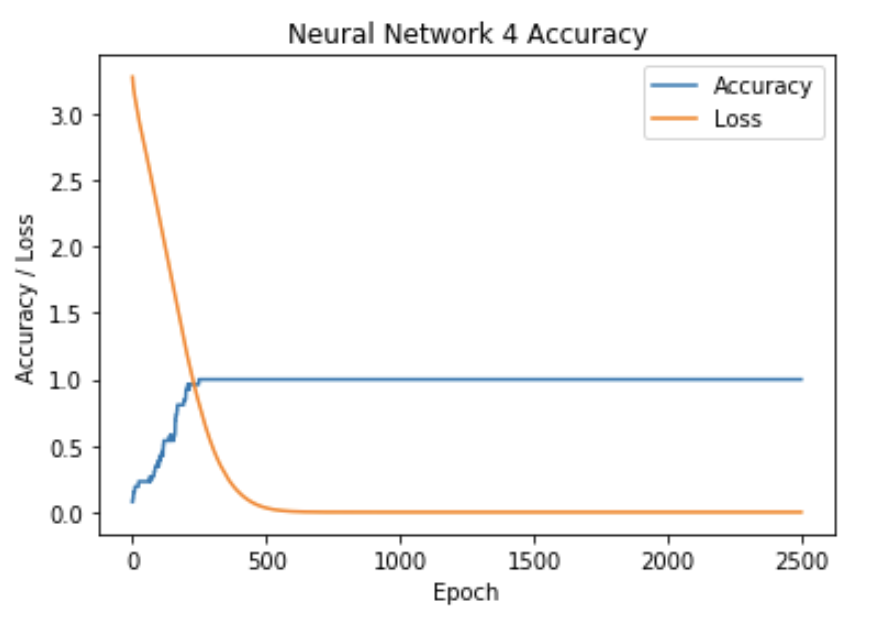
\includegraphics[width=3.4in]{figures/nn4 plot.png}
	\caption[]{Neural Network 4 Training Results} 
	\label{test4c}
\end{figure}

This model reached 100\% accuracy in 249 epochs, a decrease of 75\%, with a total training time of 13.48 seconds. 
There was a slight increase in training time, 1.10 seconds, because of number of parameters being adjusted.

\begin{figure}[!htb] \centering
	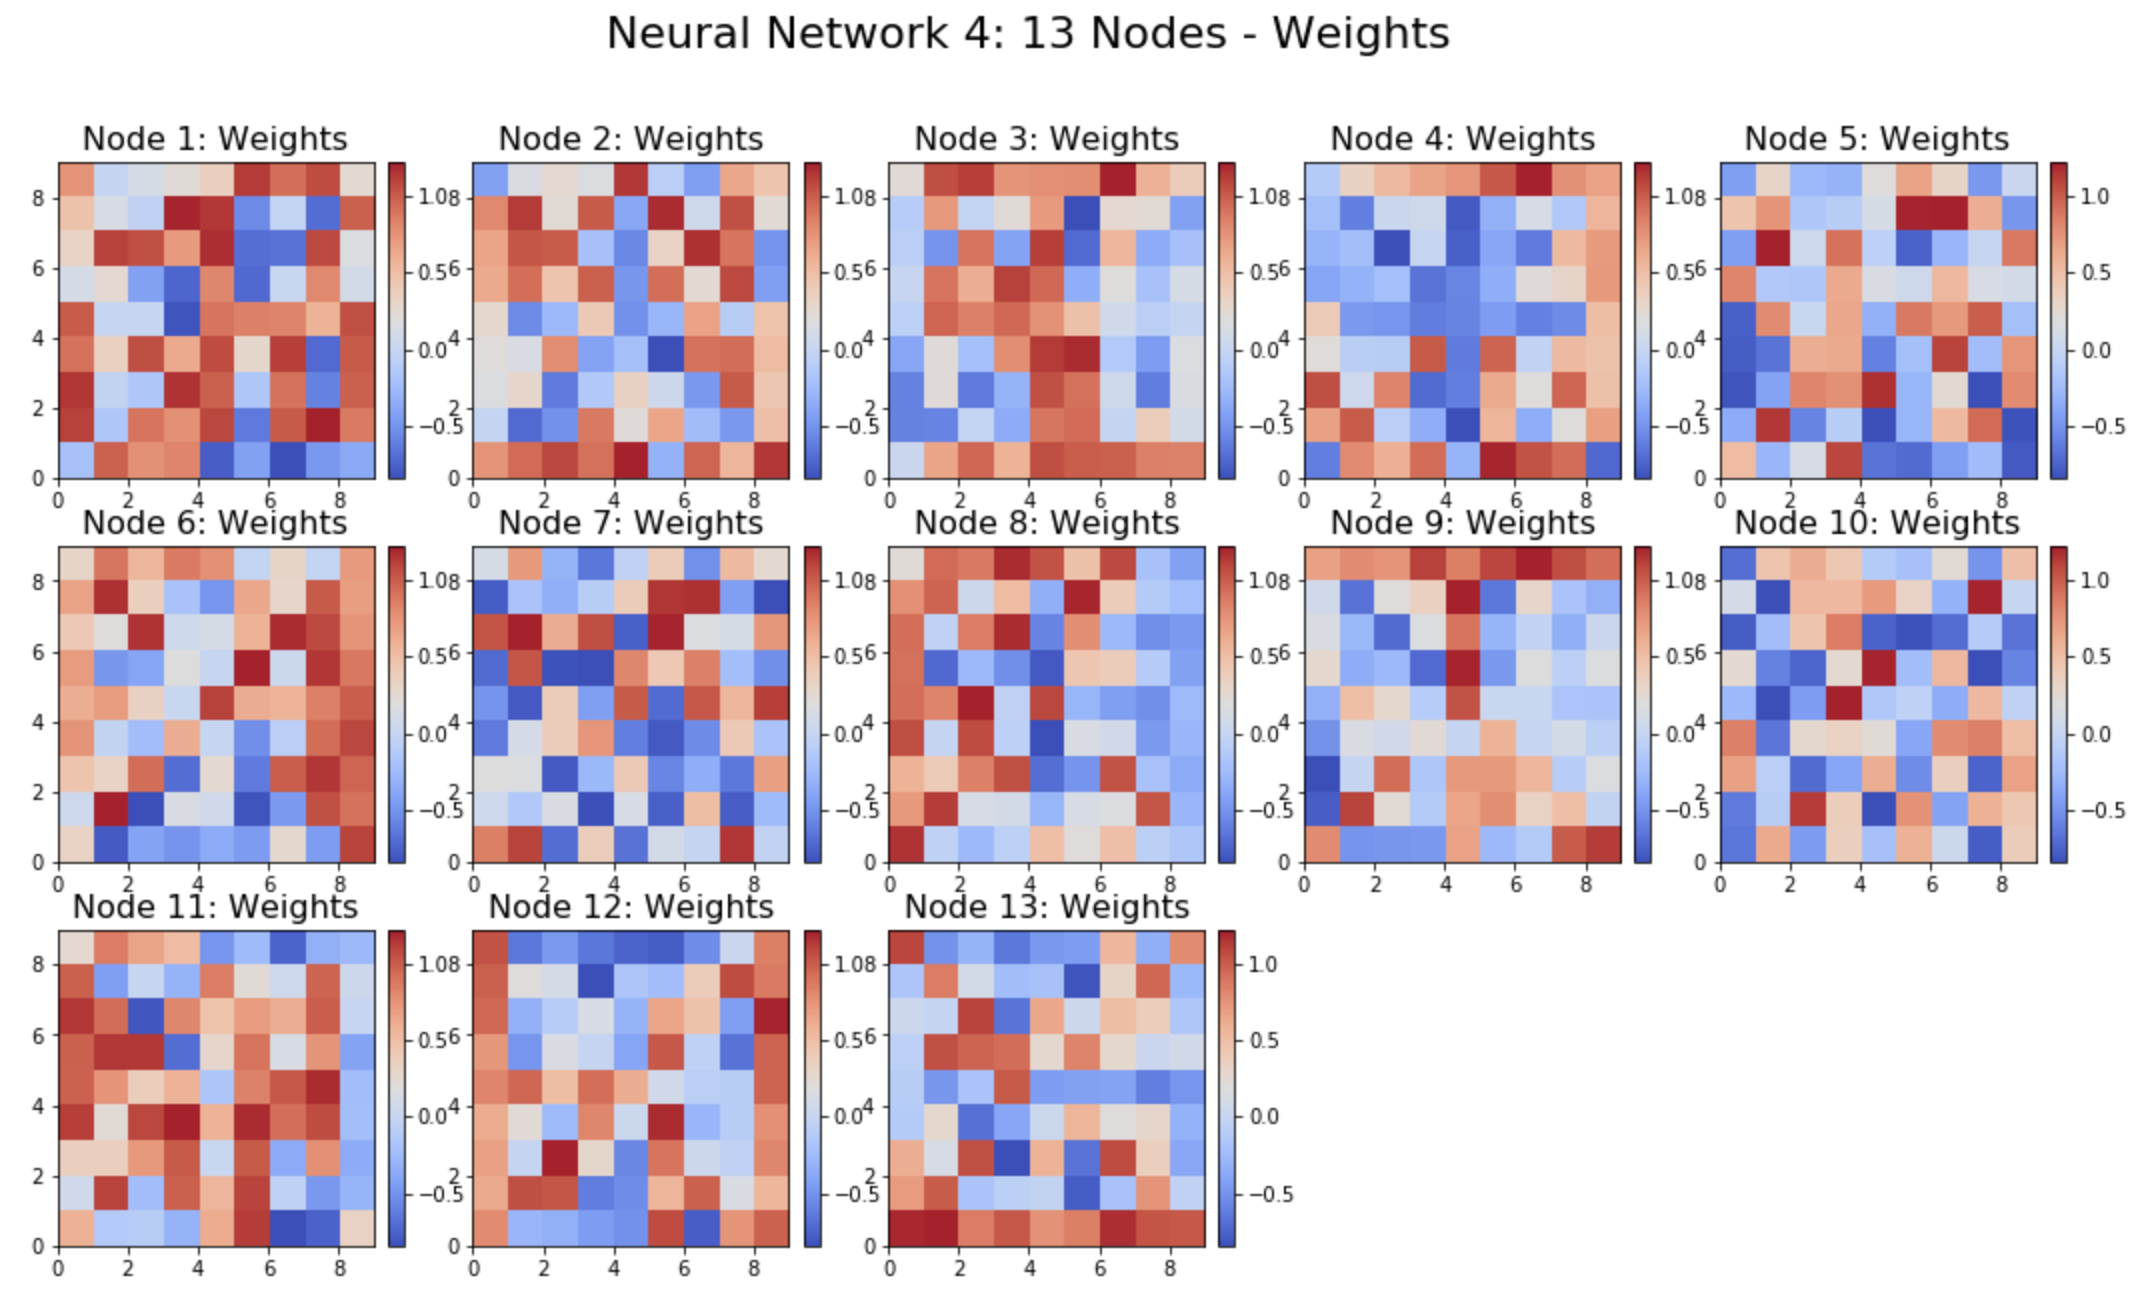
\includegraphics[width=3.4in]{figures/nn4_weights.png}
	\caption[]{Neural Network 4 Node Weights} 
	\label{test4d}
\end{figure}

Now that there are more nodes, searching for predictive signals in the dataset can become even more challenging for humans to interpret the weightings. 
There are many similarities between nodes and many differences. 
It is really difficult to key in on specific pixels.


\subsection{Neural Network 5: 26 Hidden Nodes}\label{one}

The final neural network developed for this analysis has a node for every output class. 
The 81 input variables will be compressed into 26 nodes and then proceed to the 26 output classes. 
There are now 2,834 total parameters in this model with 2,312 of them in the hidden layer and 702 in the output layer.

\begin{figure}[!htb] \centering
	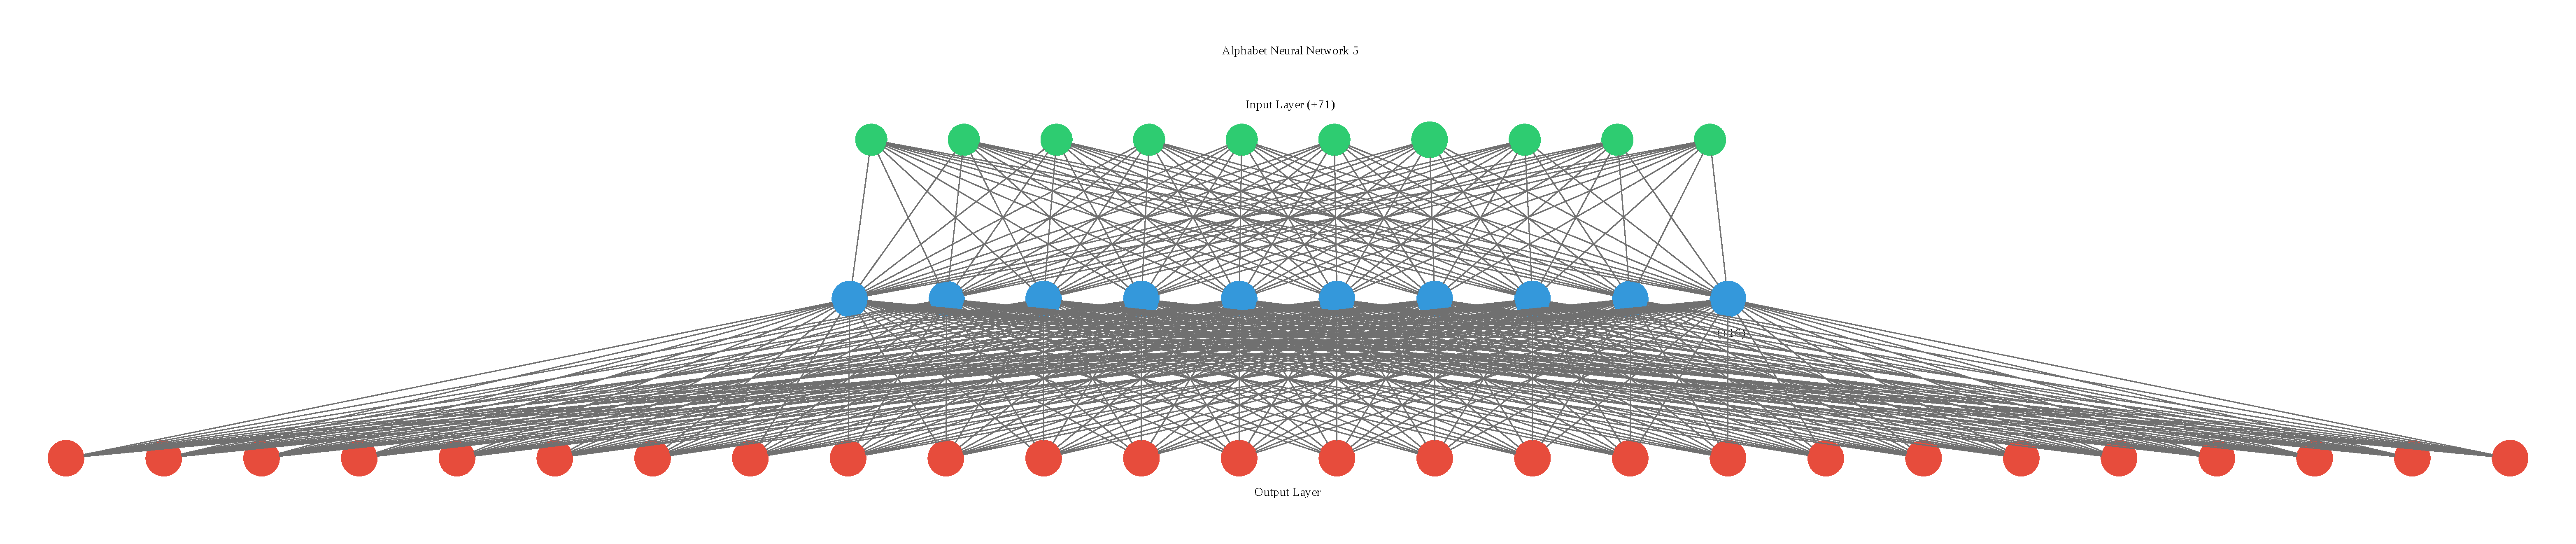
\includegraphics[width=3.4in]{figures/nn5.pdf}
	\caption[]{Neural Network 5 Architecture} 
	\label{test5a} 
\end{figure}


\begin{figure}[!htb] \centering
	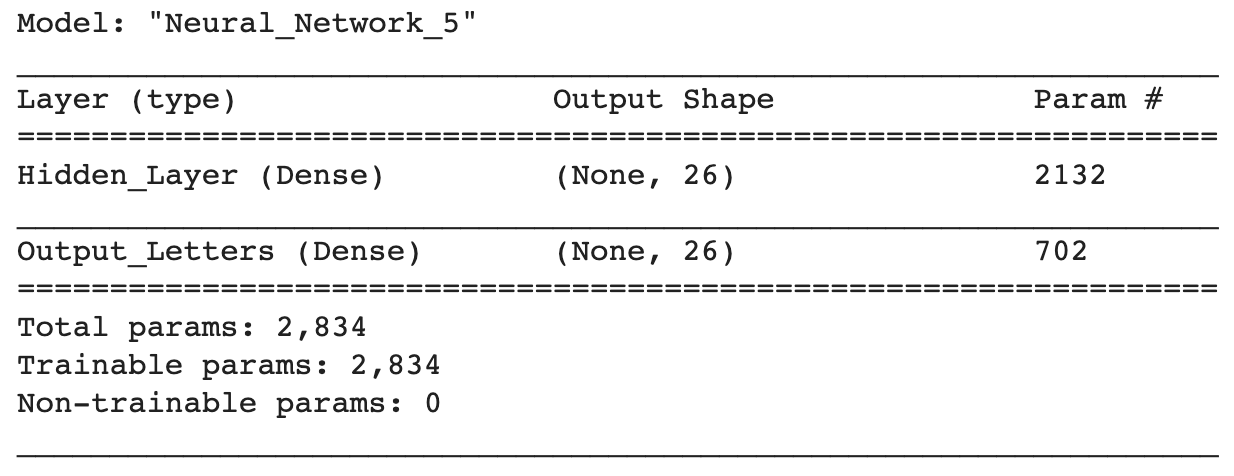
\includegraphics[width=3.4in]{figures/nn5 sum.png}
	\caption[]{Neural Network 5 Model Summary} 
	\label{test5b} 
\end{figure}

\begin{figure}[!htb] \centering
	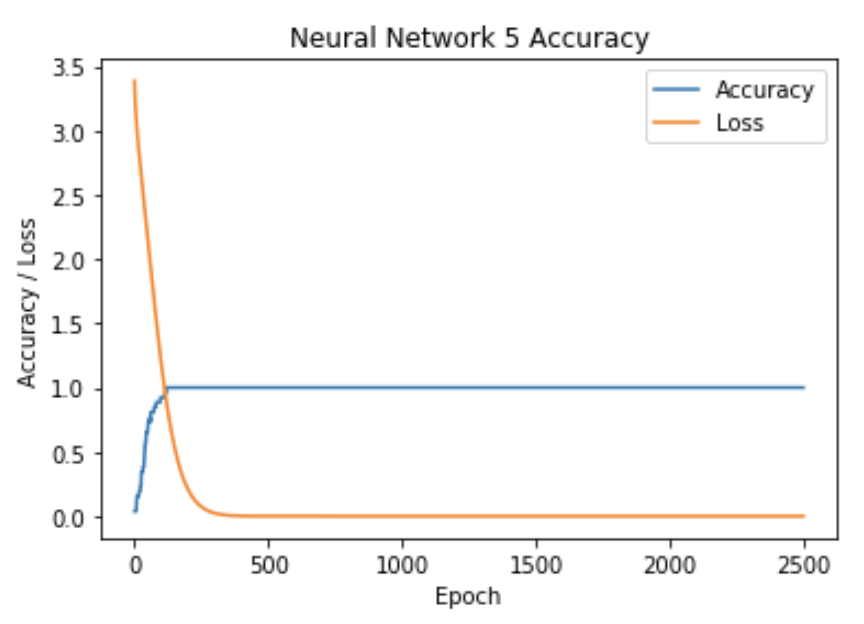
\includegraphics[width=3.4in]{figures/nn5 plot.png}
	\caption[]{Neural Network 5 Training Results} 
	\label{test5c}
\end{figure}

This model was able to reach 100\% accuracy in only 121 epochs making it the shortest number of epochs of all the models trained. 
However, this model also took the longer time to train at 15.9 seconds.

\begin{figure}[!htb] \centering
	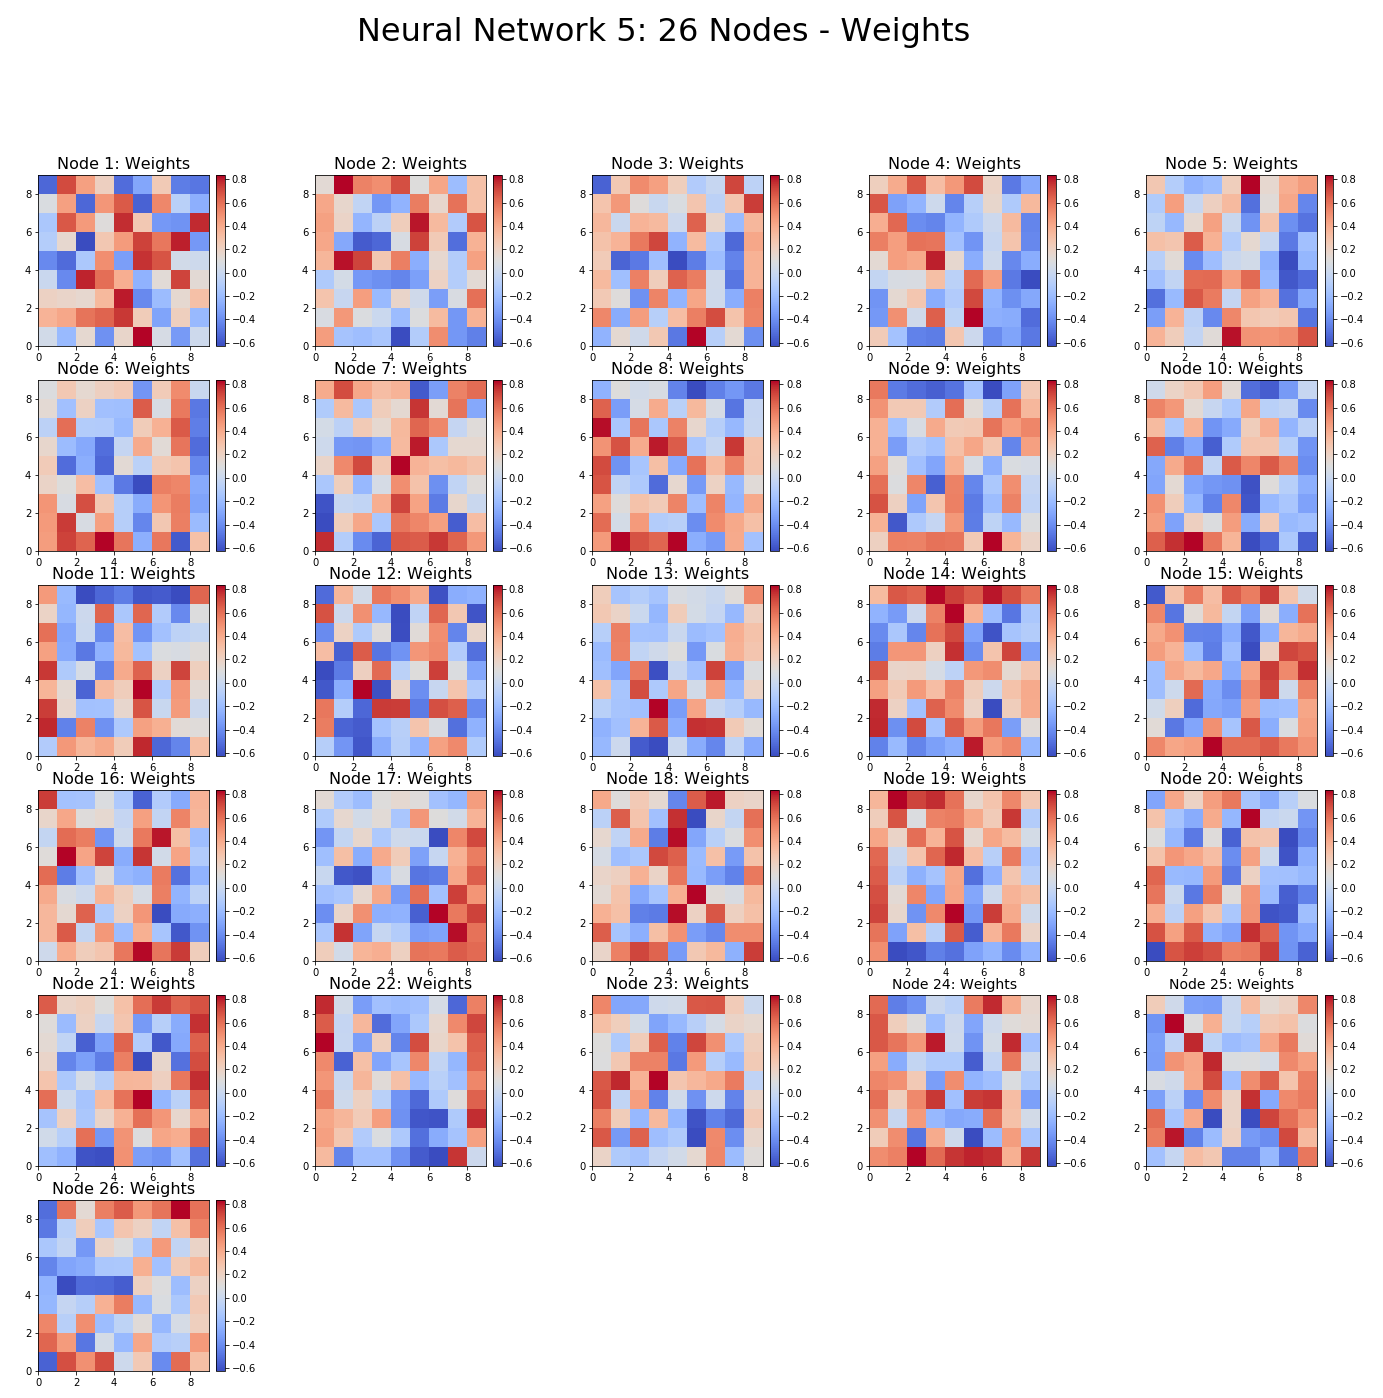
\includegraphics[width=3.4in]{figures/nn5_weights.png}
	\caption[]{Neural Network 5 Node Weights} 
	\label{test5d}
\end{figure}

The weights for each of the nodes in this model in Figure \ref{test5d} appear even more difficult to decipher than the last model. 
However, there are a handful of nodes that appear to focus on specific shapes. 
At first glance node 26 resembles the form of the letter “Z” with its positive weights. 
Almost the entire top row, bottom row, and diagonal from bottom left to top right are positively weighted. 

Certain nodes serve very specific purposes within the entire model. 
Node 13 has neutral weights over much of the area except a very concentrated 6 or 7 pixels.

\section{Discussion and Conclusion}

Each artificial neural network that was trained during this analysis accomplished the overall learning task to recognize each letter in the English alphabet. 
However, our goal to interpret the underlying feature extraction within each node in the single hidden layer was much more challenging, especially as more nodes were added. 
Even on a relatively simple neural network problem, it can be extremely challenging to see what the model is actually doing with the input dataset. 

It is clear that “black-box” algorithms, like the neural network, are more difficult to explain exactly how they used the input data to reach a given prediction. 
Understanding the mathematical processes behind the algorithm and knowing what data to include in the model can help a data scientist have confidence in their models. 
This knowledge will also allow the data scientist to properly adjust the architecture and hyperparameters within the model to achieve more accurate predictions. 


\clearpage


\bibliography{bibliographie.bib}

\bibliographystyle{newapa}

\end{document}